\documentclass[a4paper]{article}
\usepackage[margin=5mm,top=6mm,bottom=5mm]{geometry}
\usepackage{graphicx}
\usepackage{xcolor}
\definecolor{cutgray}{gray}{0.40}
\usepackage{tikz}
\pagestyle{empty}
\setlength{\parindent}{0pt}
\setlength{\parskip}{0pt}
\setlength{\tabcolsep}{1.2mm}

% Fixed mm sizes — do not use macros inside \includegraphics width=
\newcommand{\decipherkey}{%
  \begin{tikzpicture}
    \node[inner sep=0pt, outer sep=0pt] (k) at (0,0)
      {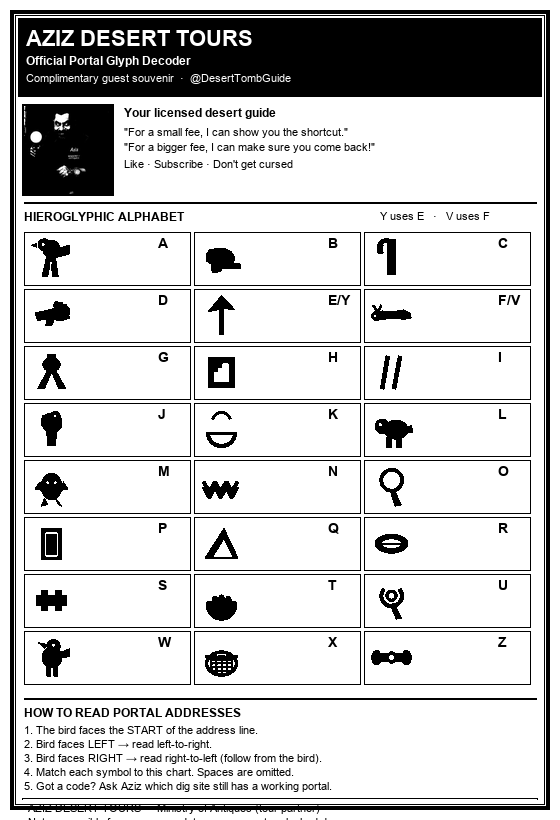
\includegraphics[width=96mm,height=132mm,keepaspectratio=false]{HieroGlyphs/brand/decipher_key_card.png}};
    \draw[cutgray, dashed, line width=0.65pt]
      (k.south west) rectangle (k.north east);
    \draw[black, line width=0.85pt]
      (k.south west) -- ++(0,3mm)
      (k.south west) -- ++(3mm,0)
      (k.south east) -- ++(0,3mm)
      (k.south east) -- ++(-3mm,0)
      (k.north west) -- ++(0,-3mm)
      (k.north west) -- ++(3mm,0)
      (k.north east) -- ++(0,-3mm)
      (k.north east) -- ++(-3mm,0);
  \end{tikzpicture}%
}

\begin{document}
\centering
{\footnotesize\bfseries Aziz Desert Tours --- Portal Glyph Decoders \quad
cut on dashed lines \quad B/W laser \quad 1 card/guest (not the real papyrus)}\\[1mm]

\begin{tabular}{@{}c@{\hspace{2mm}}c@{}}
\decipherkey & \decipherkey \\[1mm]
\decipherkey & \decipherkey \\
\end{tabular}

\newpage
\centering
{\footnotesize\bfseries Aziz Desert Tours --- extra decoder sheet (spares)}\\[1mm]
\begin{tabular}{@{}c@{\hspace{2mm}}c@{}}
\decipherkey & \decipherkey \\[1mm]
\decipherkey & \decipherkey \\
\end{tabular}

\end{document}
